\documentclass[12pt]{IEEEtran}
\usepackage{graphicx}
\usepackage{amsmath}
\usepackage{pgfplots}
\usepackage{cite}
\markboth{CPSC 530 - Information Theory and Security - Final Report - Group 17}{Last Name \MakeLowercase{\textit{et al.}}: Title}
\usepackage{filecontents}
% Insert references here
\begin{filecontents*}{references.bib}
@masterthesis{Sjostrand,
	title	= {A study in compression algorithms},
	school	= {Blekinge Institue of Technology},
	author	= {Sjostrand, Mattias Hakansson},
	year	= {2005},
	url	= {http://bth.diva-portal.org/smash/record.jsf?pid=diva2:830266}
}
\end{filecontents*}

\newcommand{\Aiden}{Aiden Taylor - B.Sc. in Computer Science}
\newcommand{\Noah}{Noah Pinel - B.Sc. in Computer Science}
\newcommand{\Ty}{Ty Irving - B.Sc. in Computer Science}

\definecolor{mybabyblue}{RGB}{140,216,231}
\definecolor{mysoftgreen}{RGB}{120,233,212}

\begin{document}
\title{The Implementation and Comparison of the BCCBT Data Compression Algorithm}
\author{
\begin{tabular}{l}
    \Aiden \\ \Noah\\ \Ty\\ 
\end{tabular}}
\date{Apr. 12th, 2023}

\maketitle

\begin{abstract}
Elaborate upon each major aspect of the paper.
\end{abstract}

\section{Introduction}
Provides the context and motivates the topic. It introduces the paper/research that is the basis of the project. \cite{Sjostrand}


\section{Proposed Work}
Describes the proposed work and evaluation framework (e.g. experiments, data analysis, statistical tests, mathematical proof..).


\section{Evaluation}
Implementation and Experiments: what you actually did (objectives, choices, data, and final analysis of results).
Base comparison: (what is a comparable work, and relating your work to existing works).
Developed software and how it can be evaluated.

\subsection{Implementation}


\subsection{Experiments}
In order to effectively be able to analyze the effectiveness of the BCCBT algorithm we had to 
find two other comparable open source compression algorithms to test against.  As a refresher for 
the factors that we had used to compare the 3 algorithms against eachother we used the 4 following
factors
\begin{enumerate}
	\item Compression Time
	\item Decompression Time
    \item Saving \% = $\frac{Orig\ File\ Size - Compressed\ File\ Size}{Orig\ File\ Size}$
    \item Compression Ratio = $\frac{Compressed\ File\ Size}{Original\ File\ Size}$
\end{enumerate}
Using these factors will enable us to effectively test whether the BCCBT algorithm is both effective 
for compressing files of differing sizes along with showing whether or not it is practical and
where the use cases for this compression algorithm.
\resizebox*{2.8in}{2.5in}{
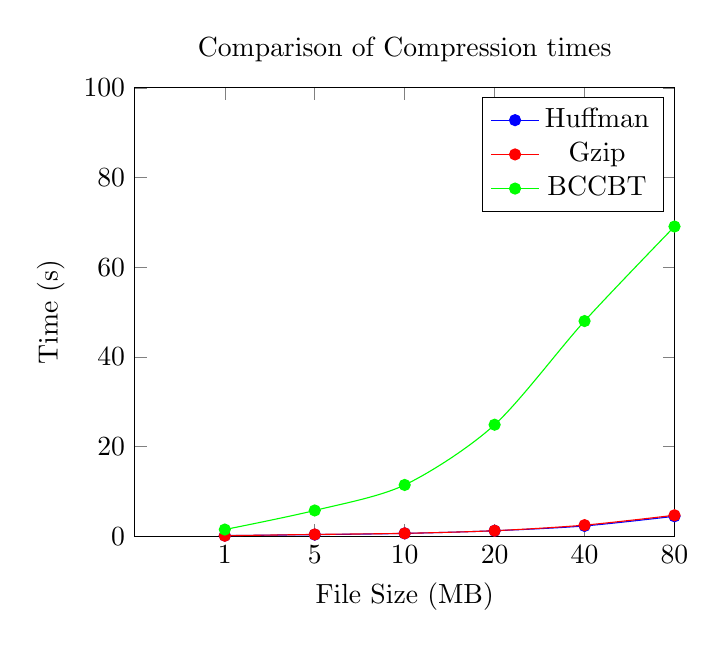
\begin{tikzpicture}
	\begin{axis}[
		xlabel=File Size (MB),
		ylabel=Time (s),
		xmin=0, xmax=6,
		ymin=0, ymax=100,
		xtick={1,2,3,4,5,6},
		xticklabels={1,5,10,20,40,80},   % <---
		ytick={0,20,...,100},
		title={Comparison of Compression times}
				]
	\addplot[smooth,mark=*,blue] plot coordinates {
		(1,0.129)(2,0.351)(3,0.625)(4,1.216)(5,2.293)(6,4.443)
	};
	\addlegendentry{Huffman}
	
	\addplot[smooth,color=red,mark=*]
		plot coordinates {
			(1,0.107)(2,0.394)(3,0.638)(4, 1.228)(5,2.472)(6, 4.671)
	
		};
	\addlegendentry{Gzip}
	\addplot[smooth,color=green,mark=*]
		plot coordinates {
			(1,1.485)(2,5.739)(3,11.430)(4,24.864)(5,47.988)(6, 69.076)
		};
	\addlegendentry{BCCBT}
	
	\end{axis}
\end{tikzpicture}}\\
These results indicate that although for low file sizes the compression time is quite similar
as the file size gets bigger the compression time exponentially gets bigger and the gap between
both Huffman and GZip gets bigger and bigger this result indicates that for the implementation
that we made it would not be practical or in your interest to use this on file sizes above 1MB
however the compression time of this algorithm can be cut down in further implementations of 
the algorithm.  Through our tests we were able to find out why the compression times of our
implementation of the BCCBT algorithm were slower than GZip and Huffman and it was due to the
population of the complete binary tree and traversing through the tree recursively rather than
iteratively which had a heavy impact on the compression time making the implementation much
slower when compared to the Huffman and Gzip compression algorithms.
\resizebox*{2.8in}{2.5in}{
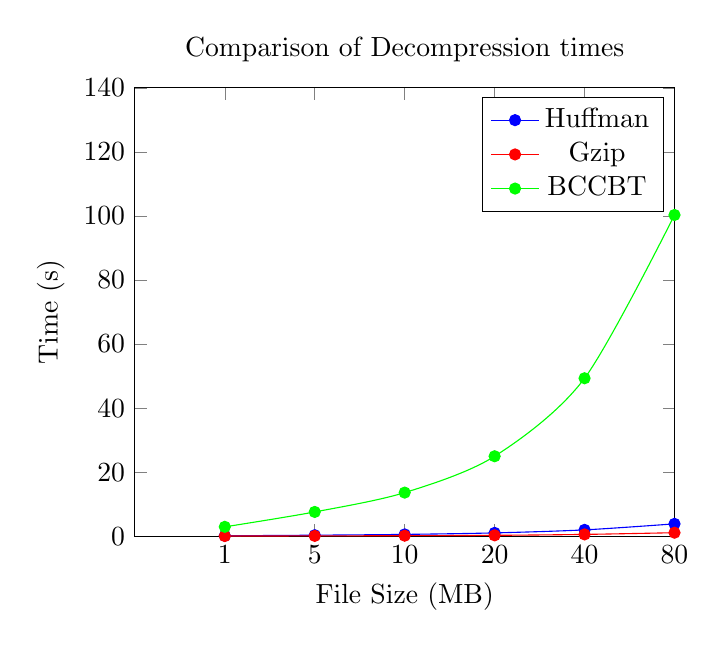
\begin{tikzpicture}
	\begin{axis}[
		xlabel=File Size (MB),
		ylabel=Time (s),
		xmin=0, xmax=6,
		ymin=0, ymax=140,
		xtick={1,2,3,4,5,6},
		xticklabels={1,5,10,20,40,80},   % <---
		ytick={0,20,...,140},
		title={Comparison of Decompression times}
				]
	\addplot[smooth,mark=*,blue] plot coordinates {
		(1,0.123)(2,0.313)(3,0.561)(4,1.030)(5,1.974)(6, 3.853)
	};
	\addlegendentry{Huffman}
	\addplot[smooth,color=red,mark=*]
		plot coordinates {
			(1,0.045)(2,0.092)(3,0.154)(4, 0.269)(5,0.557)(6, 1.091)
	
		};
	\addlegendentry{Gzip}
	\addplot[smooth,color=green,mark=*]
		plot coordinates {
			(1,2.92)(2,7.576)(3,13.611)(4,24.964)(5, 49.321)(6, 100.311)
		};
	\addlegendentry{BCCBT}
	\end{axis}
\end{tikzpicture}}\\
The results for the comparision of the decompression times are quite similar to the 
compression times mainly because while decompressing we use the similar functions to the 
compression for the files this graph also represents the problem with the optimization of
the compression and decompression of the implementation of the BCCBT algorithm while at higher
file sizes.\\
\resizebox*{2.8in}{2.5in}{
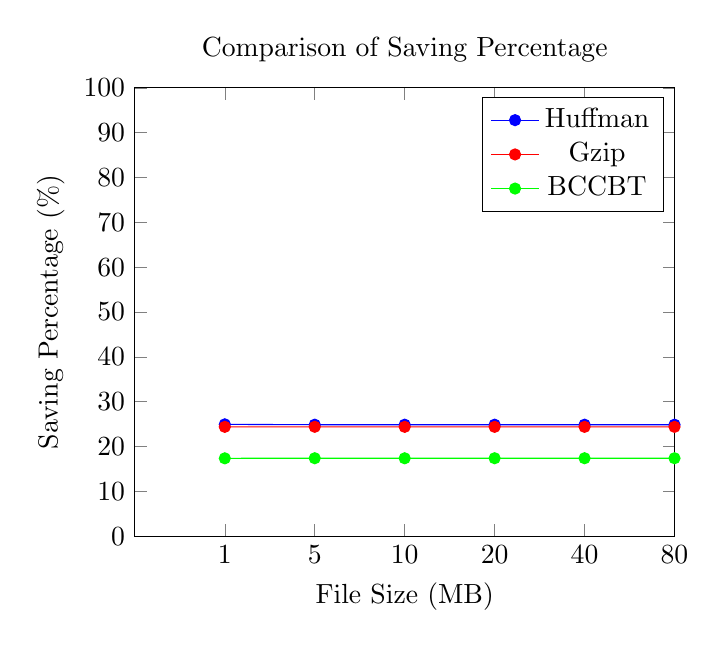
\begin{tikzpicture}
	\begin{axis}[
		xlabel=File Size (MB),
		ylabel=Saving Percentage (\%),
		xmin=0, xmax=6,
		ymin=0, ymax=100,
		xtick={1,2,3,4,5,6},
		xticklabels={1,5,10,20,40,80},   % <---
		ytick={0,10,...,100},
		title={Comparison of Saving Percentage}
				]
	\addplot[smooth,mark=*,blue] plot coordinates {
		(1,24.95)(2,24.87)(3,24.87)(4,24.87)(5,24.87)(6,24.87)
	};
	\addlegendentry{Huffman}
	
	\addplot[smooth,color=red,mark=*]
		plot coordinates {
			(1,24.39)(2,24.40)(3,24.39)(4,24.39)(5,24.39)(6,24.39)
		};
	\addlegendentry{Gzip}
	\addplot[smooth,color=green,mark=*]
		plot coordinates {
			(1,17.37)(2,17.39)(3,17.38)(4,17.39)(5,17.39)(6,17.39)
		};
	\addlegendentry{BCCBT}
	
	\end{axis}
\end{tikzpicture}}\\
The graph above demonstrates the saving percentage in \% which shows the 
comparision of the different algorithms for compression and the overall
effectiveness of each one depending on file size, this demonstrates that
the saving percentage is linear and the gap between the algorithms do not
end up becoming bigger unlike the compression/decompression times.

\resizebox*{2.8in}{2.5in}{
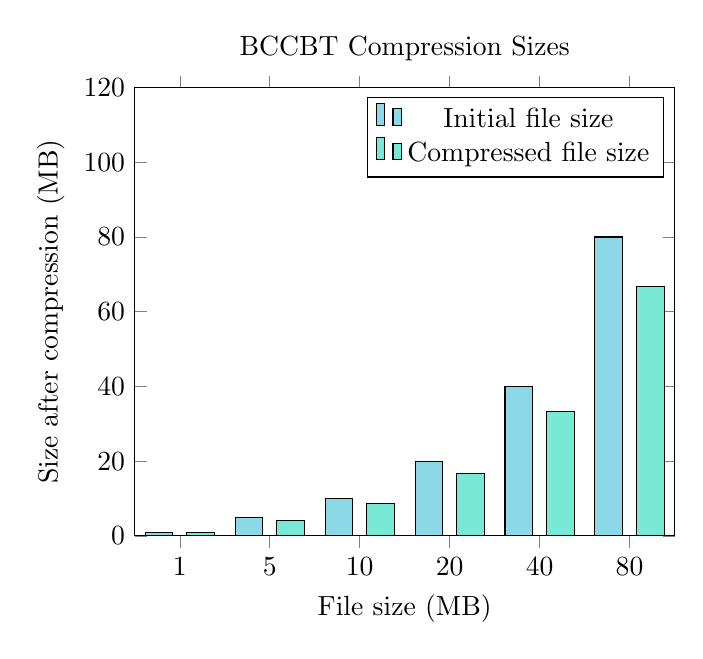
\begin{tikzpicture}
	\begin{axis}[
		title={BCCBT Compression Sizes},
		xlabel={File size (MB)},
		ylabel={Size after compression (MB)},
		ymin=0, ymax=120,
		ytick={0,20,40,60,80,100,120},
		xtick={1,2,3,4,5,6},
		xticklabels={1,5, 10, 20, 40, 80},
		ybar=5pt,
		bar width=10pt,
	]
	
	\addplot[
		fill=mybabyblue,
		]
		coordinates {
		(1,1)(2,5)(3,10)(4,20)(5,40)(6,80)
		};
		\addlegendentry{Initial file size}
		
	\addplot[
		fill=mysoftgreen,
		]
		coordinates {
		(1,0.8)(2,4.17)(3,8.6)(4,16.6)(5,33.3)(6,66.7)
		};
		\addlegendentry{Compressed file size}
	\end{axis}
\end{tikzpicture}}

\resizebox*{2.8in}{2.5in}{
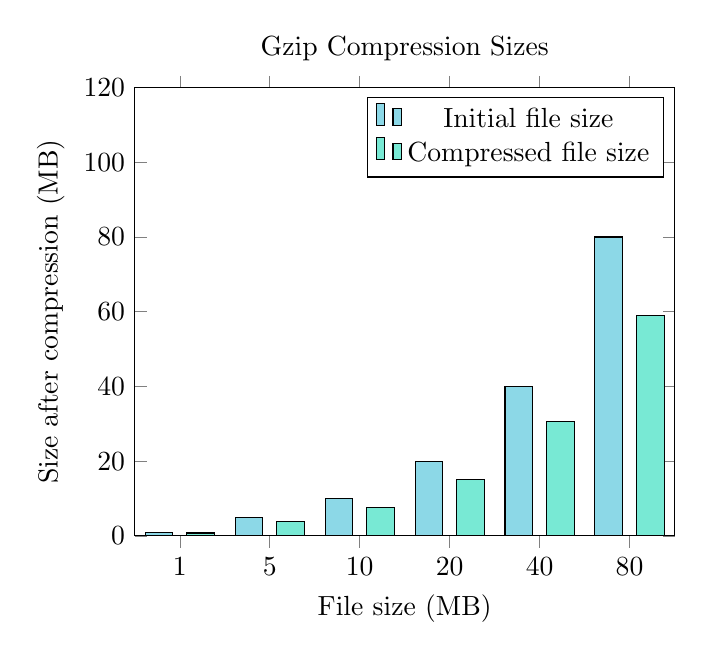
\begin{tikzpicture}
\begin{axis}[
	title={Gzip Compression Sizes},
	xlabel={File size (MB)},
	ylabel={Size after compression (MB)},
	ymin=0, ymax=120,
	ytick={0,20,40,60,80,100,120},
	xtick={1,2,3,4,5,6},
	xticklabels={1,5, 10, 20, 40, 80},
	ybar=5pt,
	bar width=10pt,
]

\addplot[
	fill=mybabyblue,
	]
	coordinates {
	(1,1)(2,5)(3,10)(4,20)(5,40)(6,80)
	};
	\addlegendentry{Initial file size}
	
\addplot[
	fill=mysoftgreen,
	]
	coordinates {
	(1,0.76)(2,3.8)(3,7.6)(4,15.2)(5,30.5)(6,59)
	};
	\addlegendentry{Compressed file size}
\end{axis}
\end{tikzpicture}}

\resizebox*{2.8in}{2.5in}{
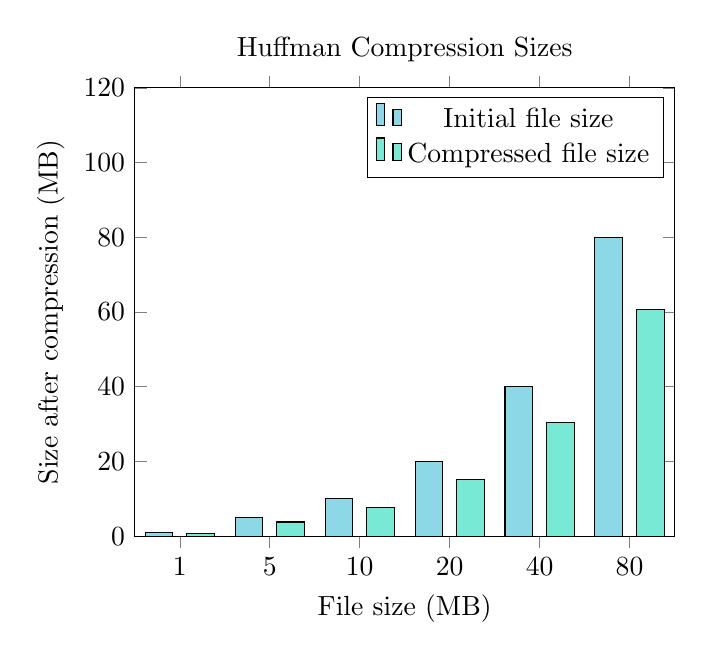
\begin{tikzpicture}
\begin{axis}[
	title={Huffman Compression Sizes},
	xlabel={File size (MB)},
	ylabel={Size after compression (MB)},
	ymin=0, ymax=120,
	ytick={0,20,40,60,80,100,120},
	xtick={1,2,3,4,5,6},
	xticklabels={1,5, 10, 20, 40, 80},
	ybar=5pt,
	bar width=10pt,
]

\addplot[
	fill=mybabyblue,
	]
	coordinates {
	(1,1)(2,5)(3,10)(4,20)(5,40)(6,80)
	};
	\addlegendentry{Initial file size}
	
\addplot[
	fill=mysoftgreen,
	]
	coordinates {
	(1,0.758)(2,3.79)(3,7.58)(4,15.17)(5,30.35)(6,60.7)
	};
	\addlegendentry{Compressed file size}
\end{axis}
\end{tikzpicture}}\\
The compression size graphs for the Huffman, Gzip, and BCCBT all show that no matter
what the file size is the amount the file size is being reduced by stays linear.  Another
important part to note about the graph is that the BCCBT does not make the compressed file size
as small as the other compression algorithms further indicating how the algorithm is not as 
efficient as the opensource algorithms that we had compared our implementation against. In conclusion
based on the experiment results that have been presented the BCCBT algorithm is a efficient 
compression algorithm however the implementation that compresses and decompresses the bitcodes,
lvls, and frequency files make the distinction of usability clear as the implementation of the 
BCCBT algorithm performs much slower making it less practical for high file sizes.
\section{Planning and Execution}
Compares the final work with the project proposal: comments on if the stated goals have been achieved, and if not, outlines the challenges.
Outlines contributions of group members including, ideas, implementation, research, writing report.

\bibliographystyle{IEEEtran}
\bibliography{references}

\end{document}
